% \cleardoublepage
% \chapter*{Introduction}
% \markboth{Introduction}{Introduction}
% \addcontentsline{toc}{chapter}{Introduction}

\chapter{Introduction}

\section{Problem and Motivation}

Suppose we are given samples of data say $\mathbf{x}$ and $\mathbf{y}$, s.t.

\begin{align*}
    \mathbf{x} = x_1, ..., x_n  \\
    \mathbf{y} = y_1, ..., y_n 
\end{align*}

For example, we may be measuring the blood pressure and heart rate of Alice at time $k$, 
say $x_k$ and $y_k$ respectively, with $x_k, y_k \in \R$. Further, suppose we are unaware of her context, for example,
Bob hacked into Alice's Apple watch and so can only read $\mathbf{x}$ and $\mathbf{y}$ --- he has no idea of 
anything she might be up to.

Bob then observes the following trend:

\begin{figure}[htb]
    \centering
    \begin{tikzpicture}
        \node (img)  {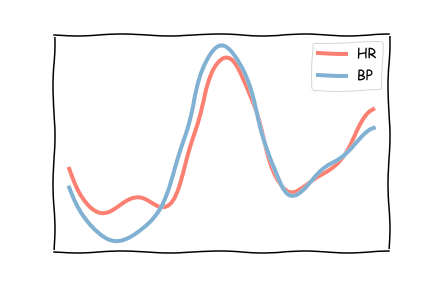
\includegraphics[width=.45\textwidth]{correlated_hr.png}};
        \node[below=of img, node distance=0cm, yshift=1cm,font=\color{black}] {time};
        \node[left=of img, node distance=0cm, rotate=90, anchor=center,yshift=-0.7cm,font=\color{black}] {bpm/mmHg};
    \end{tikzpicture}
    \caption{Heart rate (HR) and Blood pressure (BP) measured in bbp and mmHg resp.}
\end{figure}

Bob, having studied data science, is well aware of the fallacy of the law of small numbers\footnote{
    The law of small numbers is the error of concluding too much from too few data. 
}. He therefore checks again the data the next day at a slightly different time. He again observes 
a similar trend, and is now more confident in the existence of a causal relation and --- having neglected biology --- 
makes the conjecture that either blood pressure causes heart rate, or 
perhaps the other way around. 

Given this strong correlation, Bob asserts that he may either model $x$ as a function of $y$ or the other way 
around. He proceeds to find some $f$ s.t. $f(x) \approx y$. The next day, to his dismay, he notices that his
model has terrible performance when evaluated on new data. He then proceeds to see what is going on, and 
observes the following:

\begin{figure}[htb]
    \centering
    \begin{tikzpicture}
        \node (img)  {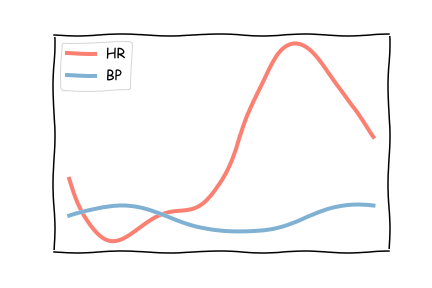
\includegraphics[width=.45\textwidth]{uncorrelated_hr.png}};
        \node[below=of img, node distance=0cm, yshift=1cm,font=\color{black}] {time};
        \node[left=of img, node distance=0cm, rotate=90, anchor=center,yshift=-0.7cm,font=\color{black}] {bpm/mmHg};
    \end{tikzpicture}
    \caption{Heart rate (HR) and Blood pressure (BP) measured in bbp and mmHg resp.}
\end{figure}

As it turns out, in the last few days, Alice was working hard on finishing her thesis and the deadline had been 
the previous day. But how, Bob wondered, could this have changed the relationship between BP and HR? 
Finally, admitting to himself that curve fitting alone is not enough to understand the world; 
Bob spends some time learning about the heart. It turns out, that fear triggers a "flight or fight"
response that increases both the heart rate and blood pressure; Interestingly your heart rate and blood pressure 
won’t always rise and fall in sync.

So what did Bob learn\footnote{
    Note that heart rate and blood pressure are intimately linked, and the story between them is more complicated.
    The plots were randomly generated using a Gaussian process, however they do resemble some real examples that 
    can be found in the internet.
}?

\begin{enumerate}
    \item When we train a model with some data, and then use it on some newly acquired data, we might
    face a \textbf{covariate-shift}\footnote{Another way to describe the covariate-shift is as follows, 
    suppose we observe some samples, but
    these samples only represent a small portion of the data space, then when we acquire new data, this new data might be very 
    different from our original acquisition. } --- that is, the distribution might change due to the context changing.
    \item When we see correlation it might be spurious due to a \textbf{confounder} --- fear was the \textbf{confounder} 
    of the heart rate and blood pressure.
\end{enumerate}

If Bob was able to incorporate these notions into his machine learning models, then it might have been more
robust to the covariate-shift. To give a more concrete example, there is a "neural net tank urban legend"\footnote{
    More about this story here: https://www.gwern.net/Tanks.
}
, where a neural network accurately predicts if there is a tank or not in an image, but it turns out it uses the 
weather as a predictor. From this it is clear that the model will perform badly under covariate shift, and indeed
it makes the case that incorporating causality to a model should make it more robust as
\cite{scholkopf2019causality} argues. Note that this is in effect the issue with generalization in machine learning:
how can we ensure that we learn \textit{meaningful} representations (features about the tanks) rather than just
correlations (the weather) useful for train accuracy. 

As for confounders, it is impossible to say anything in general\footnote{
    For most of the 20th century, a huge debate took place to determine the question of whether or not 
    smoking caused cancer. A clever argument against a causal relation was that there existed a gene that 
    made a person both want to smoke and more prone to cancer; even the father of modern statistics
    himself thought this explanation more plausible (For a good read on how science is and was used 
    for wrong see the excellent book \cite{NaomiMerchants}).
    
}. We must therefore specify a causal model, and
then see what guarantees we can give under what assumptions. Even in the absence of confounders it is highly 
non trivial to determine causality.

As this simple example illustrates, causality is related to many interesting questions; perhaps, one of the most 
simple questions we can ask --- and the one that we will explore --- is, given that either X causes Y, or Y causes X
(we assume no confounders) then, when 
can we predict the direction of causality? If yes, how? 

In the figure bellow (figure \ref{fig:simple_bivariate_example}) can you tell if $X$ causes $Y$? Or perhaps
it is the other way around? The right answer is that $X$ causes $Y$, and we will show algorithms that 
can accurately predict causality in such settings with as few as 75 samples. 

\begin{figure}[H]
    \centering
    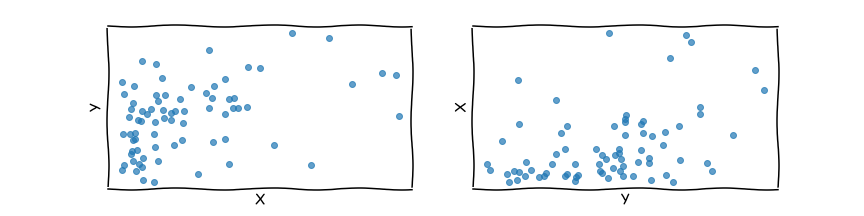
\includegraphics[width=1\textwidth]{bivariate_causal_example.png}
    \caption{75 samples of data $X$, $Y$.  The samples are generated independently as follows:
    $y_i = f(x_i) + n_i$ where $x_i$ is drawn from an exponential distribution and $n_i$ is drawn 
    independently from a Gaussian one and $f(x) = 10 \tanh(x) + 4\sin(x) + x + x^2$}
    \label{fig:simple_bivariate_example}
\end{figure}

\section{Causality}

\subsection{Causal models: FCM}

We can model any causal model by using a \textbf{Function Causal Model (FCM)} which can be constructed as follows
(\cite{Peters2017}):

We \textit{generate} a random vector\footnote{That is, each $X_i$ is a random variable.}
$X = (X_1, ..., X_d)$ by using a graph $\mathcal{G}$ (encoding the relationships),
a set of functions $f = (f_1, ..., f_d)$ (encoding the type of relationship) and a noise distribution $\mathcal{E}$
(the randomness generator).

For each $i = 1, ..., d$

$$
    X_i \leftarrow f_i(X_{\text{Pa}(i)}, E_i), \quad E_i \thicksim \mathcal{E}
$$

where $\text{Pa}(i)$ is the set of parents of $i$; and so $X_{\text{Pa}(i)}$ is the set of random variables
for the parents of $X_i$. For example in Figure \ref{fig:fcm_1}, $\text{Pa}(4) = \{1, 2\}$, 
and so $X_{\text{Pa}(4)} = \{X_1, X_2\}$.

\begin{figure}[!h]
    \centering

    \begin{tikzpicture}[
        > = stealth, % arrow head style
        shorten > = 1pt, % don't touch arrow head to node
        auto,
        node distance = 2.5cm, % distance between nodes
        thick % line style
    ]
    
    \tikzstyle{every state}=[
        draw = black,
        thick,
        fill = white,
        minimum size = 4mm
    ]
    
    \node[state] (a) {$X_1$};
    \node[state] (b) [right of=a] {$X_2$};
    \node[state] (c) [below left of=a] {$X_3$};
    \node[state] (d) [below right of=a] {$X_4$};
    
    \path[->] (a) edge node {} (c);
    \path[->] (a) edge node {} (d);
    \path[->] (b) edge node {} (d);
    
    \end{tikzpicture}
    \caption{ Example for FCM with $X = X_1, ... X4$, with $E_i \thicksim \mathcal{E}$, 
    with $X_1 = f_1(E_1)$, $X_2 = f_2(E_2)$, $X_3 = f_3(X_1, E_3)$, and 
    $X_4 = f_4(X_1, X_2, E_4)$}
    \label{fig:fcm_1}

\end{figure}


Note that causal relations can also be \textit{cyclic}, i.e. $X$ causes $Y$ which in turn causes 
$X$ ad infinitum; while this deserves consideration as many systems have feedback loops we will
for simplicity not look at such settings.

\subsection{Interventions}

To make precise the meaning of causality, suppose that we are given 
two random variables $X$, $Y$ with joint distribution $p_{x, y}$. Intuitively we 
would say that $X$ causes $Y$, or $X \rightarrow Y$, if we intervene on $X$ and then see an effect on $Y$. In particular
we will denote $\operatorname{do}(x)$ --- short for $\operatorname{do}(X = x)$ --- as an intervention
that forces the variable $X$ to have the value $x$, and leaves the rest of the system untouched. 
Following the convention inspired by \cite{pearl2000causality}, 
we define the resulting distribution as $p_{y|do(x)}$.

This motivates the following definition:

\begin{definition}
    We say that $X$ \textbf{causes} $Y$ if $p_{y|do(x)} \neq p_{y|do(x^\prime)}$ for some
    $x \neq x^\prime$
\end{definition}

When we talk about $p_{y|x}$, we often say, "The chance of $y$ given that $x$ happened". This sounds similar
to $p_{y|do(x)}$; note however that "$x$ happened" and "force $X = x$" are very different. Imagine that 
there indeed was a gene that made people both prone to smoking and cancer; then if we forced someone at 
random to smoke, he would on average be less likely to have cancer than someone who smoked because he wanted to.
This also illustrates 
one of the limitations of causality: some interventions are not possible due to ethical issues.

You might have heard about randomized trials or A/B testing, these are both common ways to estimate $p_{y|do(x)}$.
For example, when developing cures, the idea of a random trial is to give experimental drugs to participants
at random. When designing new UIs to maximize user participation in apps, developers implement A/B testing, 
they assign new versions to people at random to estimate engagement. Note that in both of these, we are able 
to avoid a potential confounder by picking $x$'s at random, and "forcing" them to "do$(x)$".

Since we will restrict ourselves to the observational setting, we will not be able to perform any interventions,
which would allow us to estimate $p_{y|do(x)}$. In this setting however, in order to perform any meaningful
inference, we will need to make concessions; in particular, we will make some assumptions about 
the causal structure. If we are able to infer the causal structure in such a setting, we 
shall call it \textbf{identifiable}.

% f we have the random variables $X$, $Y$, and $Z$, then depending on how they are causaly linked, then 
% we will have different relationships between the marginals and the Pearl's "do" conditional. For example,
% if $X \rightarrow Z \rightarrow Y$, then we will have that $p_X = p_{X|do(y)}$, but $p_Y \neq p_{Y|do(x)}$. 

% Indeed, for all 6 different relations of $X$, $Y$, and $Z$ we get a different set of relationships between 
% the interventional and observational conditions. Then, assuming that we get both interventional and observational data it suffices to check to which of the 6 
% possible structure the data corresponds to (at least in theory). 

We will restrict ourselves also to the bivariate case; one big difference worth noting is that in the
multivariate setting we can test conditional independence. Using conditional independence tests 
is a very powerful method for causal inference. Suppose 
we have random variables $X$, $Y$ and $Z$, then if we can estimate that $X \bigCI Y | Z$, then it must be 
that all information between $X$ and $Y$ must flow through $Z$ (See Figure \ref{fig:conditionalIndep}).
This test alone has has now greatly reduced the space of possible causal directions between these random variables.

One can in fact generalize the conditional independence such that $X$ and the other variables are 
a collection of random variables, which gives a lot of flexibility to devise clever algorithms. 
The theory comes from graphical models, which tries to understand the relationship between 
distributions and their graphical counterparts, such as Figure \ref{fig:conditionalIndep}.
The key difference is that in graphical models we do not care about the causal direction. 
Since we will not be using any of this theory, we will not go into any detail 
(a good overview can found in \cite{bishop2006pattern}).

\begin{figure}[!h]
    \centering

    \begin{tikzpicture}[
        > = stealth, % arrow head style
        shorten > = 1pt, % don't touch arrow head to node
        auto,
        node distance = 2.5cm, % distance between nodes
        thick % line style
    ]
    
    \tikzstyle{every state}=[
        draw = black,
        thick,
        fill = white,
        minimum size = 4mm
    ]
    
    \node[state] (a) {$Z$};
    \node[state] (b) [below left of=a] {$X$};
    \node[state] (c) [below right of=a] {$Y$};
    
    \path[-] (a) edge node {} (b);
    \path[-] (a) edge node {} (c);
    
    \end{tikzpicture}
    \caption{An example of FCM with random variables $X$, $Z$ and $Y$; we leave it undirected}
    \label{fig:conditionalIndep}

\end{figure}

In some sense the two variable case is hard because we cannot use conditional independence. As we will see, 
it is not possible to distinguish causality in the general bivariate setting when only observing 
observational data; we will thus need to restrict 
the class of such models. The underlying structure behind such causal models is what is known as 
Structural Equation Models (SEM) (\cite{Peters2017}). Essentially 
it is a model specification; and the key insight is that it should not be reversible. 


\section{Proposed Methods}

We will propose a new type of inference method which exploits the i.i.d 
noise assumption; the idea is to split the data in different intervals, and then to regress each 
interval separately. In the causal direction one would expect that the residuals of each 
interval will be more homogenous\footnote{By homogenous residuals we mean that the residuals will be similar 
to each other, for example if we plot their respective histograms, these will asymptotically converge to the 
same distribution}  --- in the ANM settings, asymmetries introduced
by inversion will break the i.i.d assumption. We will conclude by 
showing that this intuition is indeed correct, by proving that the method is consistent --- 
assuming that causal discovery is indeed possible and that the additive noise is i.i.d. We will
also propose a second method, however while also consistent, it requires knowledge of the 
noise distribution, which is not a good assumption in practice. 


\section{Outline}

We will begin by formalizing further the causal framework that we will explore; we will then present an overview of 
popular methods for inference on the bivariate causal setting. Next, we will overview some notions in statistical distance 
--- as these play a central role in causal inference --- such as maximum mean discrepancy (MMD) and f-divergences. 
For the convenience of the reader we will also review some background material that will help gain a better 
intuition on the MMD. 

We will end by going over the proposed methods, and showing both theoretical guarantees and experimental results. 




